% ---
% Reemplaza parte de la sección de resultados en Docs/Technical_Report.tex.
% Entradas que lo respaldan: H-005, H-020, H-021, H-022, H-023, H-024, H-025, H-026, H-027, H-028, H-030, H-035, D-026.
% ---

\subsection{Datos, características y selección}
\label{sec:datos_caracteristicas_seleccion}

% fuente: H-020; 2_preprocesamiento_qa.csv, 2_discordantes_sensibilidad.csv
En la auditoría del preprocesamiento sobre los 3\,568 registros del conjunto de datos,
se identificaron exactamente 80 máscaras cuyas dimensiones espaciales diferían de las de su
mamografía correspondiente. Estas correspondieron a dos categorías: 78 casos de masas
escalados de forma uniforme por un factor cercano a 0.870 (0.8700 a 0.8704 tanto en filas como en columnas),
y 2 casos de calcificaciones con un ligero desplazamiento espacial. Al contrastar las anotaciones
con los recortes oficiales proporcionados en el conjunto de datos, la regla geométrica de coincidencia
se verificó al píxel en 3\,206 de 3\,213 casos evaluables (99.8\,\%). Se detectaron únicamente 7 casos
discordantes en masas (4 en entrenamiento y 3 en prueba), en los cuales la máscara y el recorte describen
extensiones disímiles de la lesión. La exclusión de los 3 casos de prueba modifica el área bajo la curva
ROC (AUC) en el conjunto de prueba de masas entre $+0.001$ y $+0.004$ a través de las cinco condiciones
evaluadas, y ninguno de estos casos forma parte de la submuestra de 200 casos de separabilidad.

% fuente: H-021; 2_preprocesamiento_qa.csv
Respecto a la topología de las máscaras binarias, 1\,464 de las 1\,696 lesiones de masas
(86.3\,\%) presentaron islas desconectadas, frente a 0 de las 1\,872 lesiones de calcificaciones.
En todos los casos de masas, la componente conexa de mayor tamaño retuvo al menos el 99.55\,\% del área total.
La supresión de componentes menores descartó una mediana de 5 píxeles por máscara (con un valor máximo
de 110 píxeles, equivalente al 0.45\,\% del área de la lesión). La distancia del píxel descartado más lejano
al borde de la componente mayor presentó una mediana de 3.6 píxeles, un percentil 99 de 9.2 píxeles
y un máximo de 14 píxeles, lo que resulta consistente con la hipótesis de que las islas corresponden a artefactos periféricos inmediatos al contorno.

% fuente: H-023, H-024; 3_tamano_efecto.csv
En la etapa de extracción de características radiómicas sobre el conjunto de entrenamiento
(637 lesiones malignas y 681 benignas en masas; 544 malignas y 1\,002 benignas en calcificaciones),
la evaluación univariante mediante la distancia estandarizada de Cohen ($|d|$) mostró que, en las
características extraídas para este conjunto de entrenamiento, las calcificaciones alcanzan tamaños de efecto
individual superiores a los de las masas. En masas, la característica
con mayor tamaño de efecto fue \texttt{firstorder\_Maximum} con $|d| = 0.50$ (con un rango de 0.40 a 0.50
en las doce primeras), seguida de descriptores morfológicos como
\texttt{shape2D}\allowbreak\texttt{\_MinorAxisLength} ($|d| = 0.45$),
\texttt{shape2D}\allowbreak\texttt{\_MaximumDiameter} ($|d| = 0.44$)
y \texttt{shape2D}\allowbreak\texttt{\_MajorAxisLength} ($|d| = 0.43$). Por su parte, en calcificaciones
la característica más discriminativa fue \texttt{shape2D}\allowbreak\texttt{\_MinorAxisLength} con $|d| = 0.82$
(con un rango de 0.64 a 0.82 en las doce primeras), seguida de \texttt{shape2D}\allowbreak\texttt{\_Perimeter} ($|d| = 0.71$).

% fuente: H-023, H-024; 3_tamano_efecto.csv
En el subconjunto de masas se observó que los primeros puestos del ordenamiento corresponden a
características de primer orden calculadas sobre intensidades sin calibrar (\texttt{Maximum}, \texttt{90Percentile},
\texttt{Energy}, \texttt{Median} y \texttt{Mean}). Dado que la base de datos combina digitalizadores sin consignar
el fabricante en los metadatos correspondientes, no es posible descartar que parte de dicha señal provenga de
diferencias en la adquisición física de la imagen. Adicionalmente, el ordenamiento univariante directo en masas
seleccionó 7 características de primer orden y 5 morfológicas sin incluir ninguna variable de textura
(0 de matrices de coocurrencia GLCM y 0 de matrices de longitud de rachas GLRLM), exhibiendo una correlación
media intercaracterística de $|r| = 0.61$ con 8 pares por encima de $|r| > 0.95$, además de duplicados exactos
en dos dimensiones tales como \texttt{Energy} y \texttt{TotalEnergy}, o \texttt{MeshSurface} y \texttt{PixelSurface} ($r = 1.0000$).
En calcificaciones, el conjunto preliminar incluyó 1 característica de primer orden, 2 morfológicas, 4 de GLCM
y 5 de GLRLM, con una correlación media de $|r| = 0.58$ y 5 pares con $|r| > 0.95$.

% fuente: H-025; 3_efecto_clahe.csv
La aplicación de ecualización adaptativa de histograma con limitación de contraste (CLAHE)
reordenó las lesiones con una correlación de Spearman cercana a 0.84 respecto a las intensidades crudas,
pero no aportó ganancia discriminativa neta. La variación mediana en $|d|$ fue de $-0.002$ en masas
y de $-0.010$ en calcificaciones. Las características de intensidad de primer orden sufrieron una reducción
mediana de $|d|$ de $-0.031$ en masas y de $-0.054$ en calcificaciones, compensada únicamente por incrementos
menores en descriptores de textura (GLRLM $+0.011$ en masas, GLCM $+0.014$ en calcificaciones), sin mejorar
el poder de separación de las características dominantes (figuras~\ref{fig:m3_effect_sizes} y~\ref{fig:m3_clahe_effect}).

\begin{figure}[htbp]
\centering
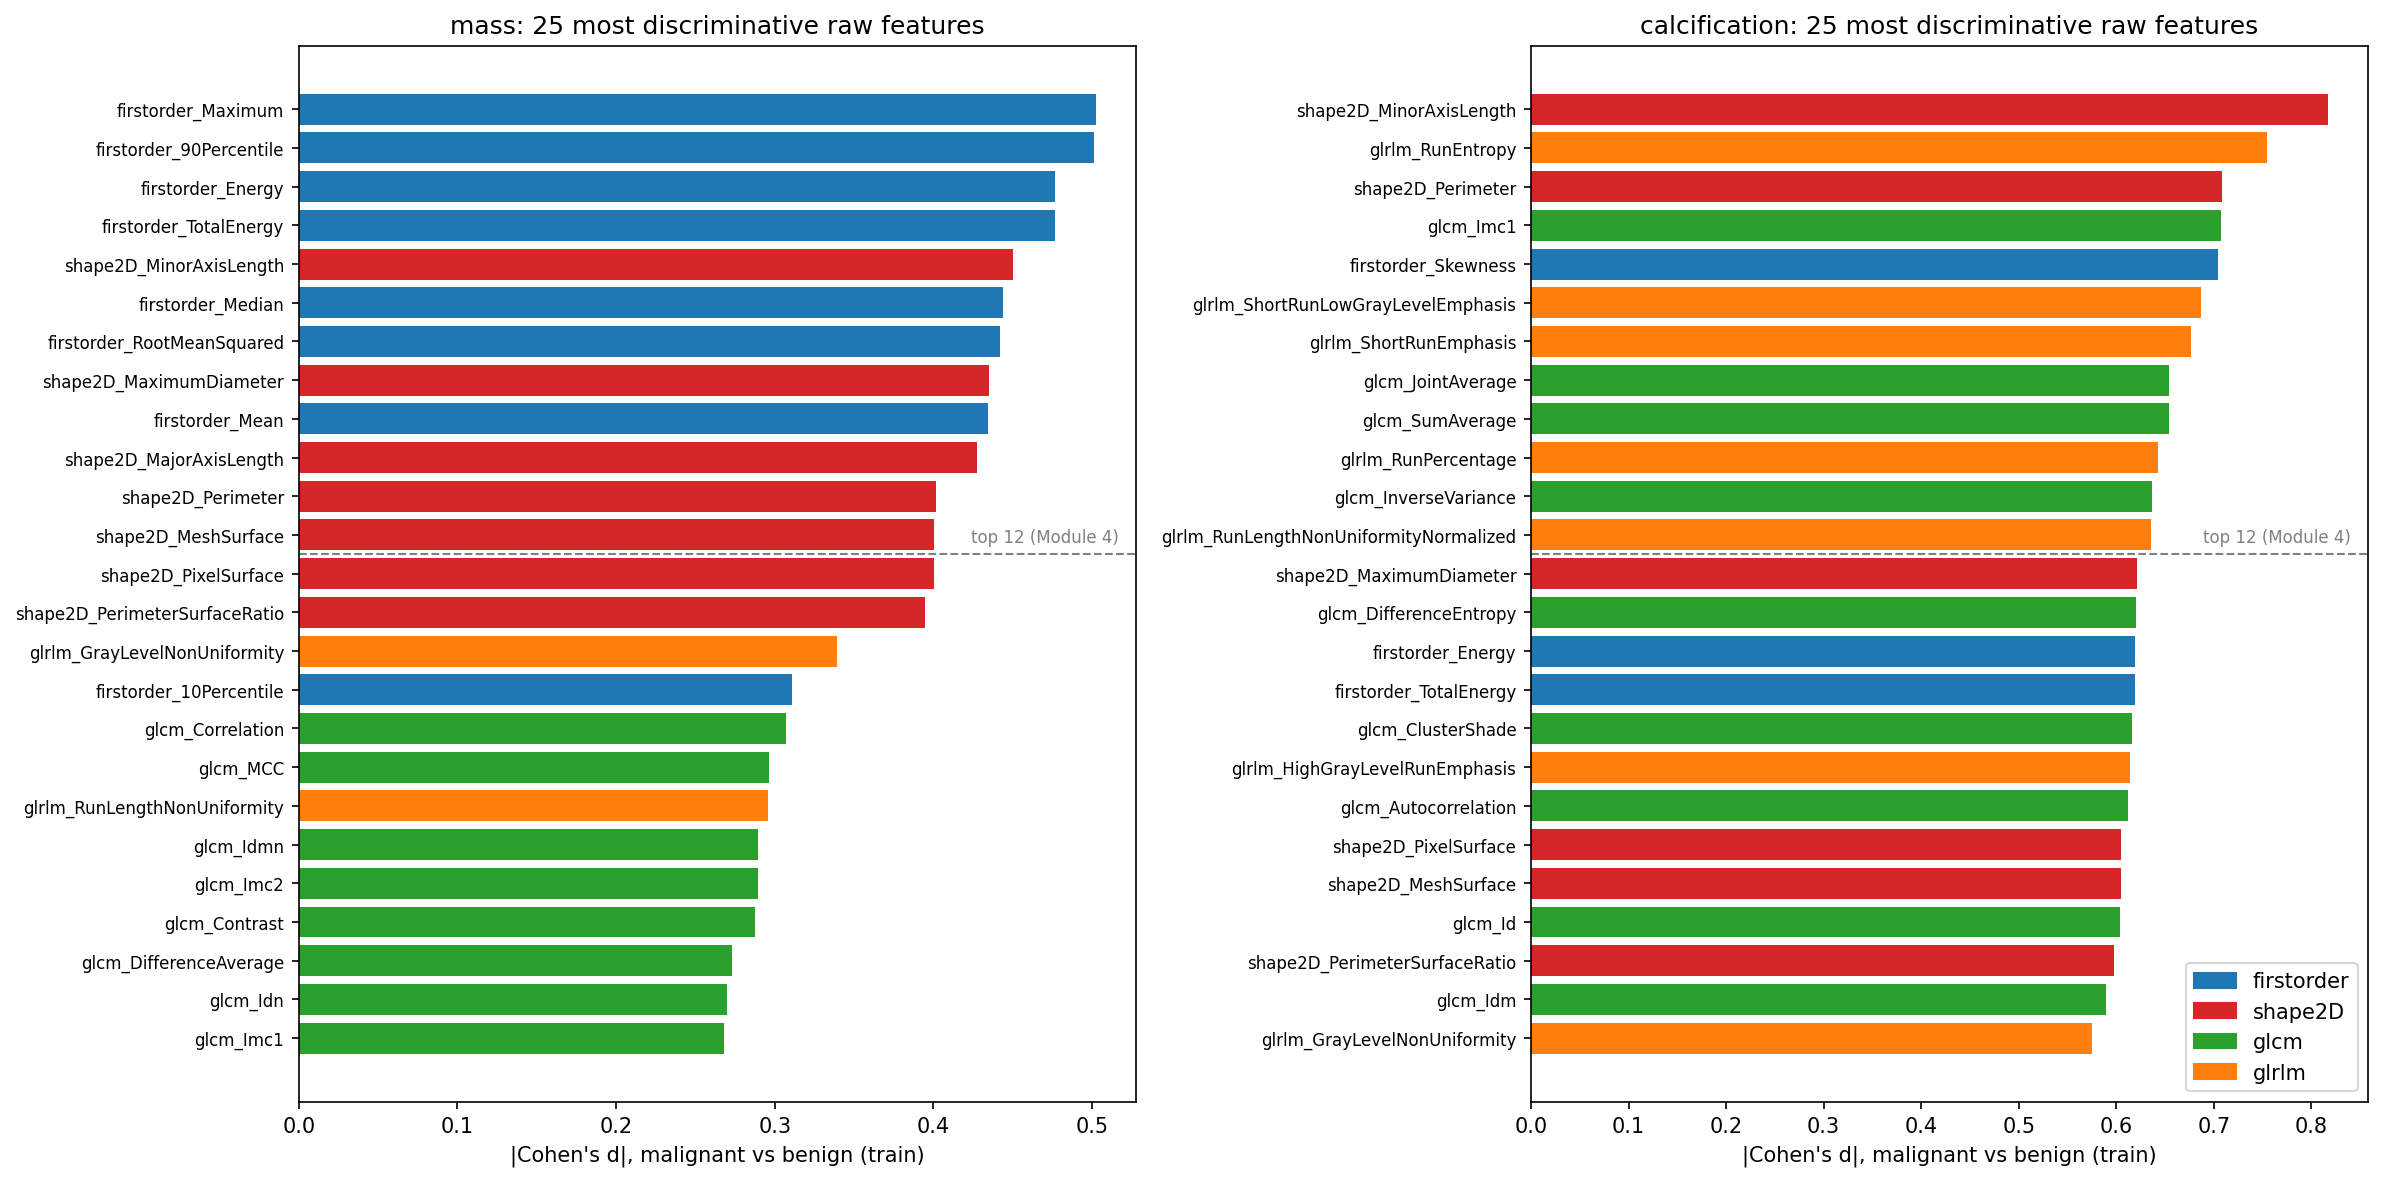
\includegraphics[width=\textwidth]{Figures/M3_effect_sizes.png}
% fuente: H-023; 3_tamano_efecto.csv
\caption{Tamaños de efecto de Cohen ($|d|$) para las características radiómicas evaluadas en el conjunto de entrenamiento de masas y calcificaciones.}
\label{fig:m3_effect_sizes}
\end{figure}

\begin{figure}[htbp]
\centering
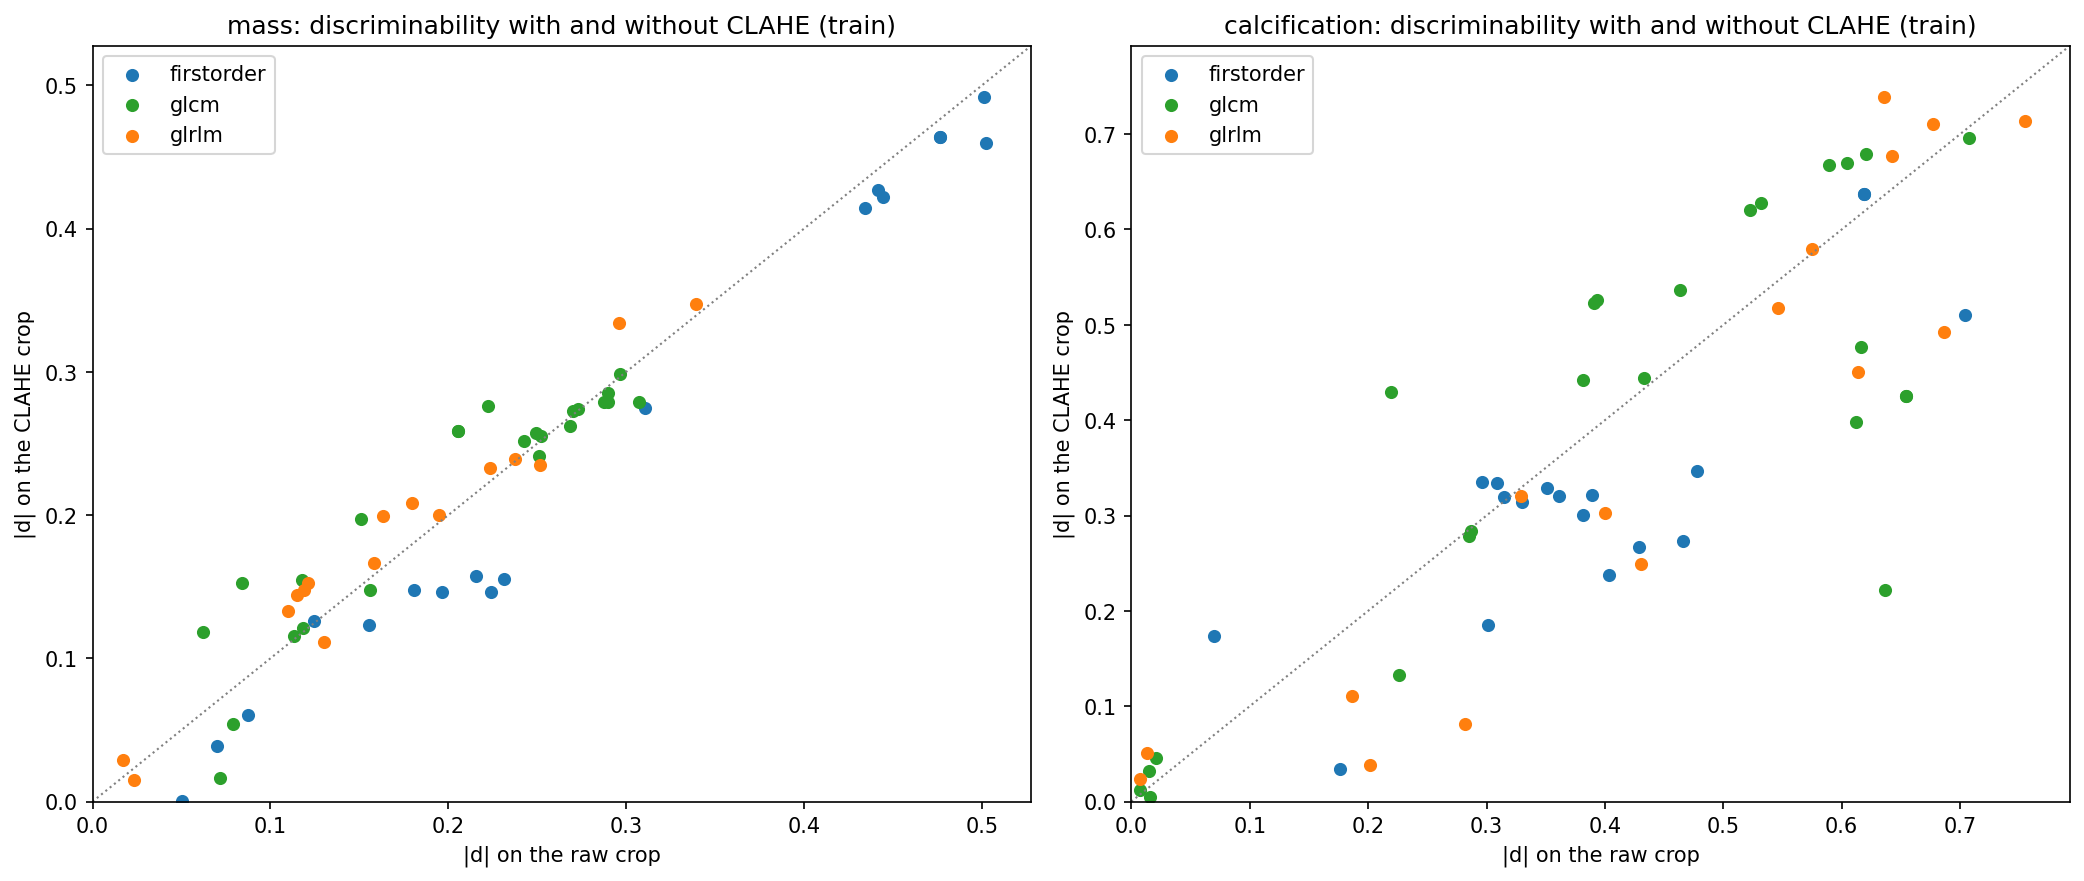
\includegraphics[width=\textwidth]{Figures/M3_clahe_effect.png}
% fuente: H-025; 3_efecto_clahe.csv
\caption{Efecto de la ecualización CLAHE sobre la capacidad discriminativa y el reordenamiento de características radiómicas por familia.}
\label{fig:m3_clahe_effect}
\end{figure}

% fuente: H-026; 4_seleccion.csv, 4_descartadas_redundancia.csv, 4_sensibilidad_umbral.csv
Para la selección final a doce características, la incorporación de la restricción de redundancia
($|r| \le 0.95$) descartó 7 variables redundantes en masas y 8 en calcificaciones, eliminando los duplicados
analíticos. En masas, la composición final se rebalanceó a 4 características de primer orden, 5 morfológicas,
1 de GLCM y 2 de GLRLM, reduciendo la correlación media a $|r| = 0.50$ y el valor máximo a $|r| = 0.94$.
La entrada de descriptores de textura en masas se mantuvo estable ante variaciones del umbral de correlación
entre 0.99 y 0.80. En calcificaciones, el conjunto final reunió 2 características de primer orden, 3 morfológicas,
4 de GLCM y 3 de GLRLM, con una correlación media de $|r| = 0.50$. Las doce variables resultantes se presentan
en la Tabla~\ref{tab:m4_seleccion}.

% fuente: H-026; 4_seleccion.csv
% Generado por Code/tools/tablas_latex.py desde 4_seleccion.csv. No editar a mano: volver a correr el script.
\begin{table}[H]
\centering
\small
\caption{Las 12 características seleccionadas en cada subconjunto (M4): F-test ANOVA sobre el entrenamiento con restricción de redundancia $|r| \le$ 0.95 (D-024).}
\label{tab:m4_seleccion}
\begin{adjustbox}{max width=\linewidth}
\begin{tabular}{r l l r l l r}
\toprule
 & \multicolumn{3}{c}{Masas} & \multicolumn{3}{c}{Calcificaciones} \\ \cmidrule(lr){2-4}\cmidrule(lr){5-7}
\# & Característica & Familia & $F$ & Característica & Familia & $F$ \\
\midrule
1 & firstorder\_Maximum & firstorder & 83.1 & shape2D\_MinorAxisLength & shape2D & 235.4 \\
2 & firstorder\_90Percentile & firstorder & 82.6 & glrlm\_RunEntropy & glrlm & 200.9 \\
3 & firstorder\_Energy & firstorder & 74.7 & shape2D\_Perimeter & shape2D & 177.0 \\
4 & shape2D\_MinorAxisLength & shape2D & 66.7 & firstorder\_Skewness & firstorder & 174.6 \\
5 & shape2D\_MaximumDiameter & shape2D & 62.3 & glrlm\_ShortRunLowGrayLevelEmphasis & glrlm & 166.2 \\
6 & shape2D\_Perimeter & shape2D & 53.1 & glrlm\_ShortRunEmphasis & glrlm & 161.5 \\
7 & shape2D\_MeshSurface & shape2D & 52.8 & glcm\_JointAverage & glcm & 150.9 \\
8 & shape2D\_PerimeterSurfaceRatio & shape2D & 51.3 & glcm\_InverseVariance & glcm & 142.8 \\
9 & glrlm\_GrayLevelNonUniformity & glrlm & 37.8 & glcm\_DifferenceEntropy & glcm & 135.6 \\
10 & firstorder\_10Percentile & firstorder & 31.7 & firstorder\_Energy & firstorder & 135.1 \\
11 & glcm\_Correlation & glcm & 31.0 & glcm\_ClusterShade & glcm & 133.9 \\
12 & glrlm\_RunLengthNonUniformity & glrlm & 28.8 & shape2D\_PixelSurface & shape2D & 129.1 \\
\bottomrule
\end{tabular}
\end{adjustbox}
\end{table}


% fuente: H-028; 4_seleccion.csv
En la etapa de escalado angular, el uso de escalado por valores extremos (\texttt{MinMaxScaler})
hacia el intervalo $[0, \pi]$ comprimía excesivamente las distribuciones de aquellas características con colas
pesadas. En calcificaciones, el rango intercuartílico (IQR) de \texttt{firstorder\_\allowbreak Energy} resultaba
en $0.046$\,rad (con mediana de $0.015$\,rad) y el de \texttt{shape2D\_\allowbreak PixelSurface} en $0.057$\,rad
(mediana de $0.020$\,rad), en contraste con una mediana global de IQR de $0.34$\,rad en masas y $0.40$\,rad en
calcificaciones. La adopción de una transformación por cuantiles hacia una distribución uniforme en $[0, \pi]$
permitió que las doce características en ambos subconjuntos alcanzaran de forma homogénea un IQR de $\pi/2$
($1.569$ a $1.572$\,rad; figura~\ref{fig:m4_selection_angles}).

% fuente: H-027, D-026; 4_semilla_folds.csv, 4_folds.csv
Para la partición en cinco pliegues de validación cruzada, la agrupación por paciente evitó
la fragmentación de estudios pertenecientes a un mismo individuo, la cual afectaba al 59\,\% de los pacientes
en masas y al 74\,\% en calcificaciones bajo particiones estratificadas simples. Al evaluar la partición inicial
con semilla 42, el segundo pliegue de calcificaciones exhibió un 52\,\% de casos malignos frente al 35\,\%
poblacional (desviación de 0.168). La selección mediante búsqueda sistemática entre 200 semillas identificó
la semilla 125 en masas y la semilla 168 en calcificaciones, acotando la desviación máxima de malignidad
a 0.011 en masas y a 0.019 en calcificaciones (proporciones entre 0.33 y 0.37 por pliegue).

% fuente: H-005
En cuanto a la división entre los conjuntos de entrenamiento y prueba, la auditoría de partición confirmó
la ausencia de fuga de pacientes (\textit{data leakage}) dentro de cada subproblema analizado.
En masas se contabilizaron 691 pacientes en entrenamiento y 201 en prueba sin solapamiento alguno (0 pacientes
compartidos); análogamente, en calcificaciones se identificaron 602 pacientes en entrenamiento y 151 en prueba,
igualmente con 0 solapes. A nivel global, considerando ambos hallazgos de forma conjunta, se registraron 1\,248
pacientes en entrenamiento y 349 en prueba con 31 pacientes solapados, discrepancia que se origina
porque la partición oficial del CBIS-DDSM se formuló de forma independiente para cada tipo de lesión, de modo que
un mismo individuo puede presentar masas en entrenamiento y calcificaciones en prueba. Este comportamiento
proporciona respaldo metodológico para procesar masas y calcificaciones como subproblemas
independientes, eliminando por construcción la posibilidad de contaminación entre conjuntos.

\begin{figure}[htbp]
\centering
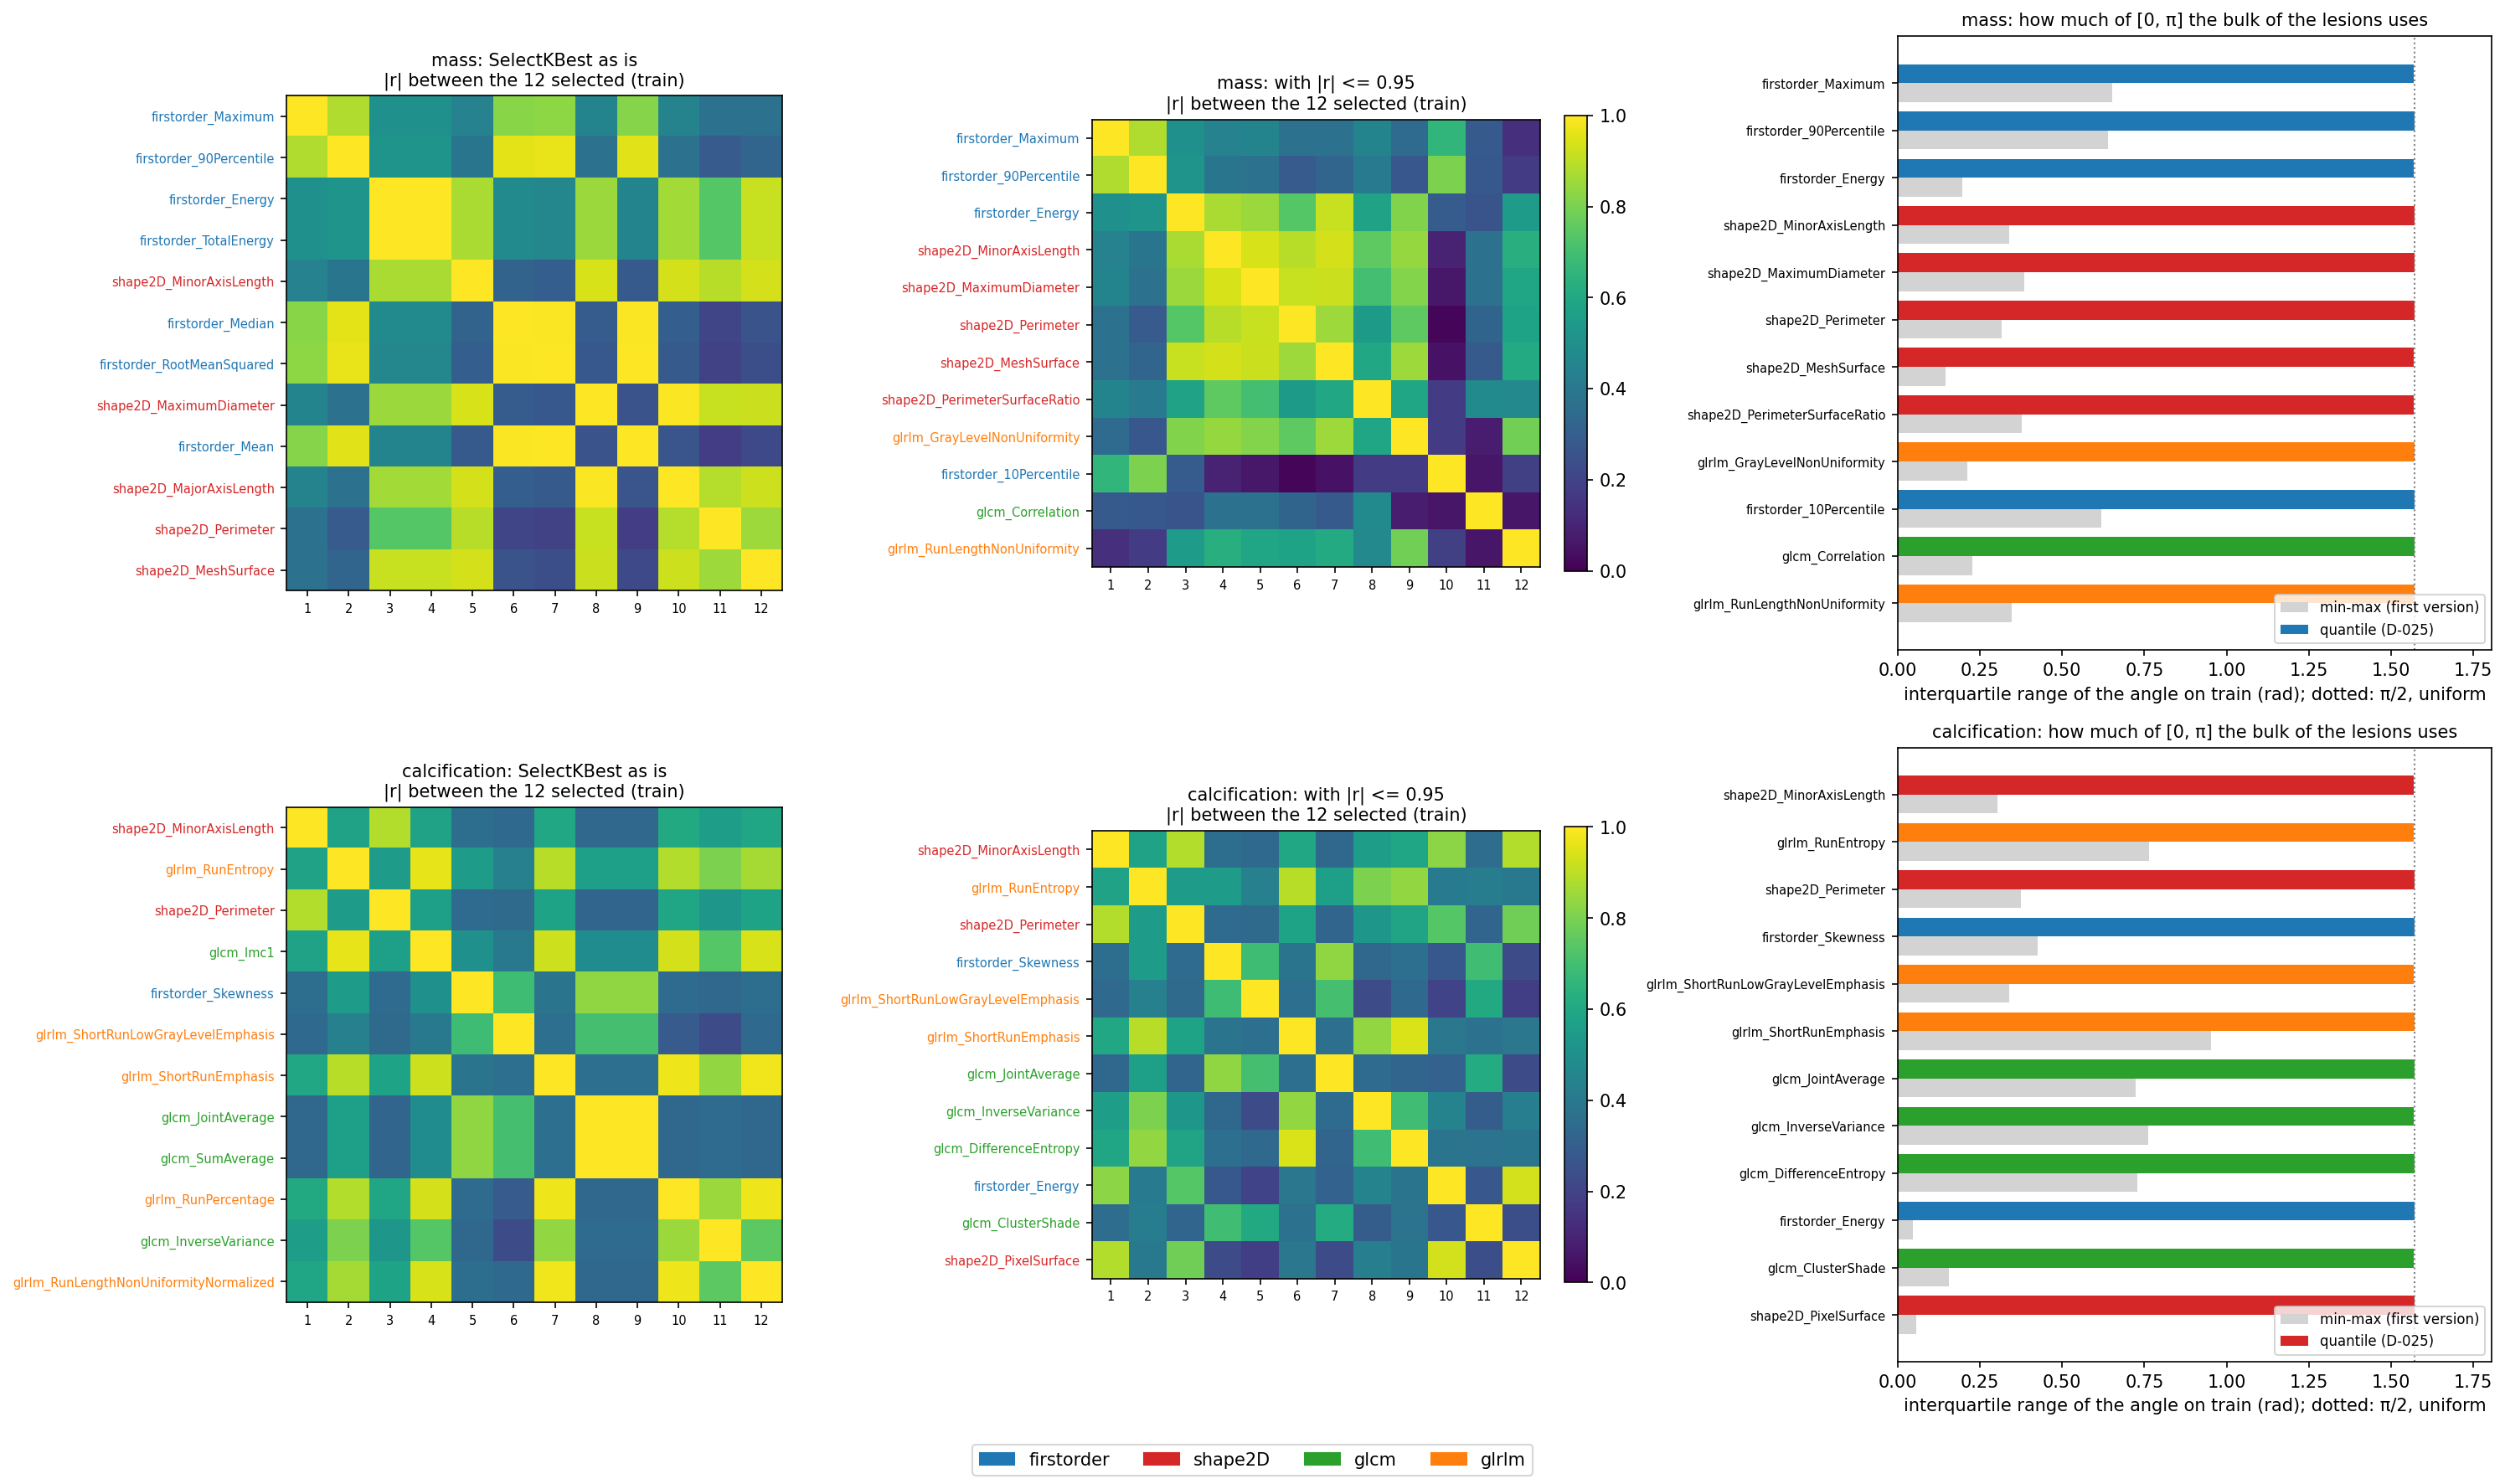
\includegraphics[width=\textwidth]{Figures/M4_selection_and_angles.png}
% fuente: H-026, H-028; 4_seleccion.csv
\caption{Distribución angular tras la selección de características y comparación entre escalado por valores extremos y transformación por cuantiles.}
\label{fig:m4_selection_angles}
\end{figure}

% fuente: H-035; X1_varianza_retenida.csv, X1_auc_por_condicion.csv, X1_auc_vs_k.csv
El análisis sobre la pérdida de información al reducir de 67 a 12 características reveló que
las variables seleccionadas retienen el 86.8\,\% de la varianza total en masas y el 90.2\,\% en calcificaciones,
frente al 98.0\,\% y 97.8\,\% alcanzable mediante las doce primeras componentes de un análisis de componentes
principales. En términos de capacidad predictiva sobre el conjunto de entrenamiento, la reducción a doce dimensiones
implicó una disminución de 2 a 4 puntos de AUC en modelos clásicos: en regresión logística, el AUC descendió
de $0.693 \pm 0.039$ a $0.650 \pm 0.056$ en masas y de $0.800 \pm 0.028$ a $0.758 \pm 0.025$ en calcificaciones;
en bosques aleatorios, la variación fue de $0.695 \pm 0.043$ a $0.680 \pm 0.046$ en masas y de $0.796 \pm 0.018$
a $0.773 \pm 0.024$ en calcificaciones. Asimismo, doce características seleccionadas al azar obtuvieron desempeños
comparables ($0.656 \pm 0.019$ y $0.659 \pm 0.023$ en masas; $0.765 \pm 0.015$ y $0.775 \pm 0.016$ en calcificaciones),
ilustrando que las variables con mayor puntuación univariante individual no necesariamente configuran el conjunto
óptimo debido a redundancias en la información compartida \cite{Guyon2003} (figura~\ref{fig:x1_selection_auc_vs_k}).

\begin{figure}[htbp]
\centering
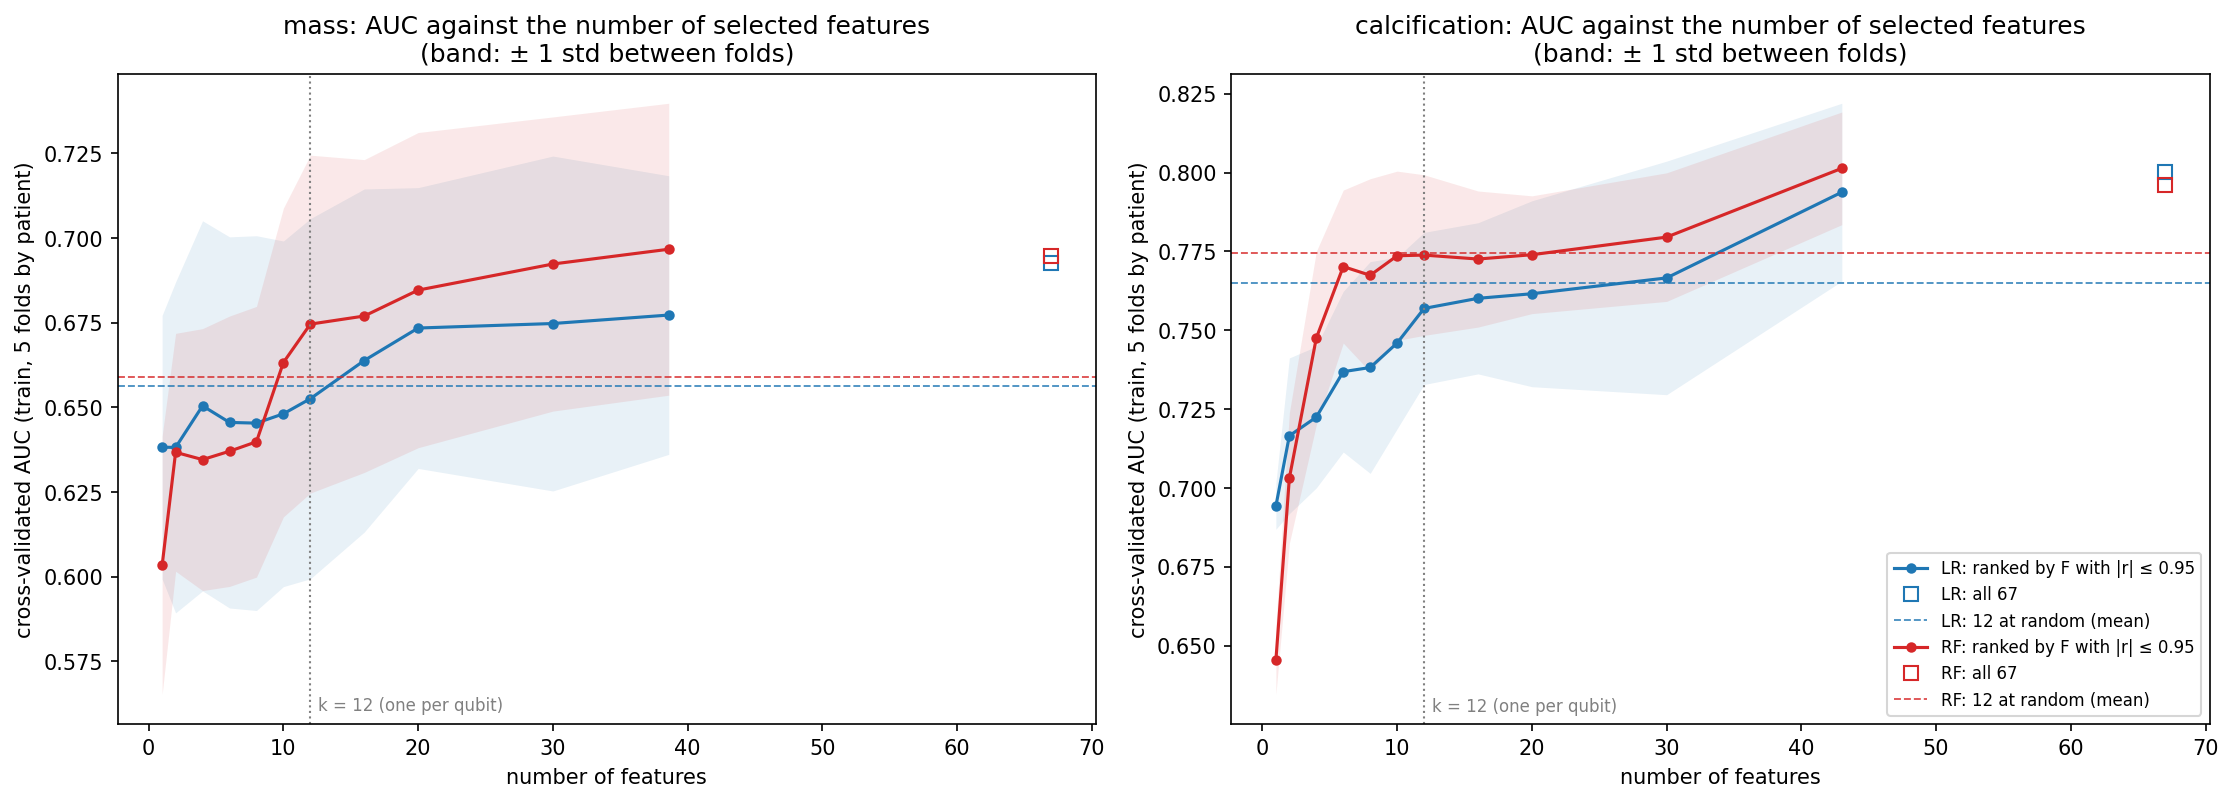
\includegraphics[width=\textwidth]{Figures/X1_selection_auc_vs_k.png}
% fuente: H-035; X1_auc_vs_k.csv
\caption{Evolución del área bajo la curva ROC en función del número de características $k$ para modelos clásicos en entrenamiento.}
\label{fig:x1_selection_auc_vs_k}
\end{figure}

% fuente: H-030, H-035
Esta limitación intrínseca de la selección univariante introduce una consideración metodológica central que matiza la comparación:
el criterio de \texttt{SelectKBest} evalúa cada variable de forma aislada mediante la prueba F de ANOVA, mientras que el filtro de
redundancia examina correlaciones lineales dos a dos. Como consecuencia, aquellas características cuyo poder discriminativo dependa
exclusivamente de interacciones de orden superior con otras variables (como en configuraciones de tipo o-exclusivo) resultan
descartadas antes de alimentar el circuito cuántico. Esta dinámica genera una tensión conceptual con el diseño experimental, puesto que
el bloque de acoplamiento $ZZ$ del mapa de características codifica precisamente productos de pares $(\pi - x_i)(\pi - x_j)$, que
constituyen el mecanismo primario mediante el cual la transformación cuántica podría aportar ventajas frente a representaciones clásicas.
Aunque la comparación entre las cinco condiciones se mantiene metodológicamente rigurosa al suministrar exactamente el mismo vector
de 12 características a todos los modelos, la ausencia de una selección multivariante capaz de capturar interacciones complejas
representa una restricción de diseño que contextualiza los resultados y explica por qué la selección guiada por F no supera de forma
concluyente a selecciones aleatorias en el experimento X1.
